\setAuthor{Jarl Patrick Paide}
\setRound{piirkonnavoor}
\setYear{2021}
\setNumber{G 6}
\setDifficulty{6}
\setTopic{TODO}

\prob{Jalgrattur}
Samal ajal, kui jalgrattur sõidab mööda kindlat teelõiku, alustab auto juhuslikul ajahetkel juhuslikust kohast sellel teelõigul sõitu. Auto sõidab jalgratturiga samas suunas, kuid kaks korda kiiremini, ning mõlemad sõidavad teelõigu lõpuni. Mis on tõenäosus, et auto sõidab jalgratturist mööda?


\hint

\solu
Joonisel punane joon kirjeldab jalgratturi asukohta $s$ ajahetkel $t$ (Rattur läbib teelõigu pikkusega $L$ aja $T$ jooksul). Auto alustab sõitu juhuslikul ajahetkel $0 < t_a < T$ ja juhuslikust kohast $0 < s_a < L$. Kui auto alustab sõitu jalgratturist eespool siis ei sõida auto jalgratturist mööda \pp{2}. Jalgrattur sõidab poole auto kiirusega. Seetõttu ei jõua auto jalgratturist mööda kui auto alustab sõitu vähemalt kaks korda kaugemal lõpule kui jalgratturi kaugus lõpuni \pp{2}. Seega auto sõidab jalgratturist mööda, kui auto alustab sõitu jalgratturist tagapool ja kui auto on jalgratturile lähemal kui jalgrattur lõppule. Vastavalt sobiv vahemik on näidatud joonisel sinise alana. Kui auto algpunkt $(t_a; s_a)$ asub sinisel alal siis sõidab auto jalgratturist mööda.

\begin{figure}[H]
  \centering
  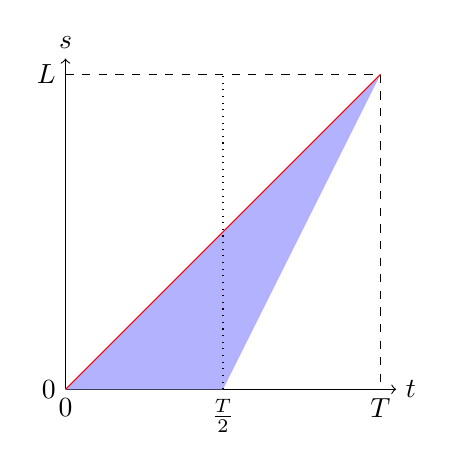
\begin{tikzpicture}[domain=0:4]
    \draw[->] (0,0) node[below] {0} -- (2,0) node[below] {$\frac{T}{2}$} -- (4,0) node[below] {$T$} -- (4.2,0) node[right] {$t$};
    \draw[->] (0,0) node[left] {0} -- (0,4) node[left] {$L$} -- (0,4.2) node[above] {$s$};
    \draw[dashed] (0,4) -- (4,4) -- (4,0);
    \fill[fill=blue!30] (0,0) -- (2,0) -- (4,4);
    \draw[dotted] (2,0) -- (2,4);
    \draw[color=red] plot (\x,\x);
  \end{tikzpicture}
\end{figure}


Tõenäosus, et auto sõidab jalgratturist mööda on võrdne sinise ala suhetega kogu pindalasse.
$$\frac{(L\times \frac T2)/2}{L \times T} = \frac{1}{4} \quad \pp{6}$$

Alternatiivselt saab vastuse leida ka ilma jooniseta. Sellisel juhul anda punkte arvutuste eest järgnevalt. Tõenäosus, et auto alustab sõitu jalgratturist eespool on $\frac{1}{2}$ \pp{2}. Tõenäosus, et auto alustab sõitu jalgratturist tagapool ja ei möödu jalgratturist on $\frac{1}{4}$ \pp{3}. Seega tõenäosus, et auto sõidab jalgratturist mööda on  $\frac{1}{4}$ \pp{1}.
\probend